\subsection{Experiment-1. 12.02.2020}\label{experiment-1.-12.02.2020}

The first attempt took place on 12.02.2020.

The aim was to involve as many UEs as possible. This is the reason for performing the experiment on that day. Eventually, \textbf{6 UEs} took part ranging by the Android version from 4 to 9.

Besides, the installation of apps and binding Wi-Fi to the necessary
access point, a detailed \textbf{journal of the Wi-Fi} connection
information enabled. This allowed monitoring RSS value on each UE.

\subsection{Weather conditions}

\begin{itemize}
\tightlist
\item
  no precipitation
\item
  cloudy sky
\item
  a thin layer of snow on the ground
\item
  temperature of -1..+1$^\circ$
\end{itemize}

\subsection{Procedure}

All items of the experiment placed on the carton boxes on the ground, so that they are a bit raised from the ground.

\begin{figure}[H]
	\centering
	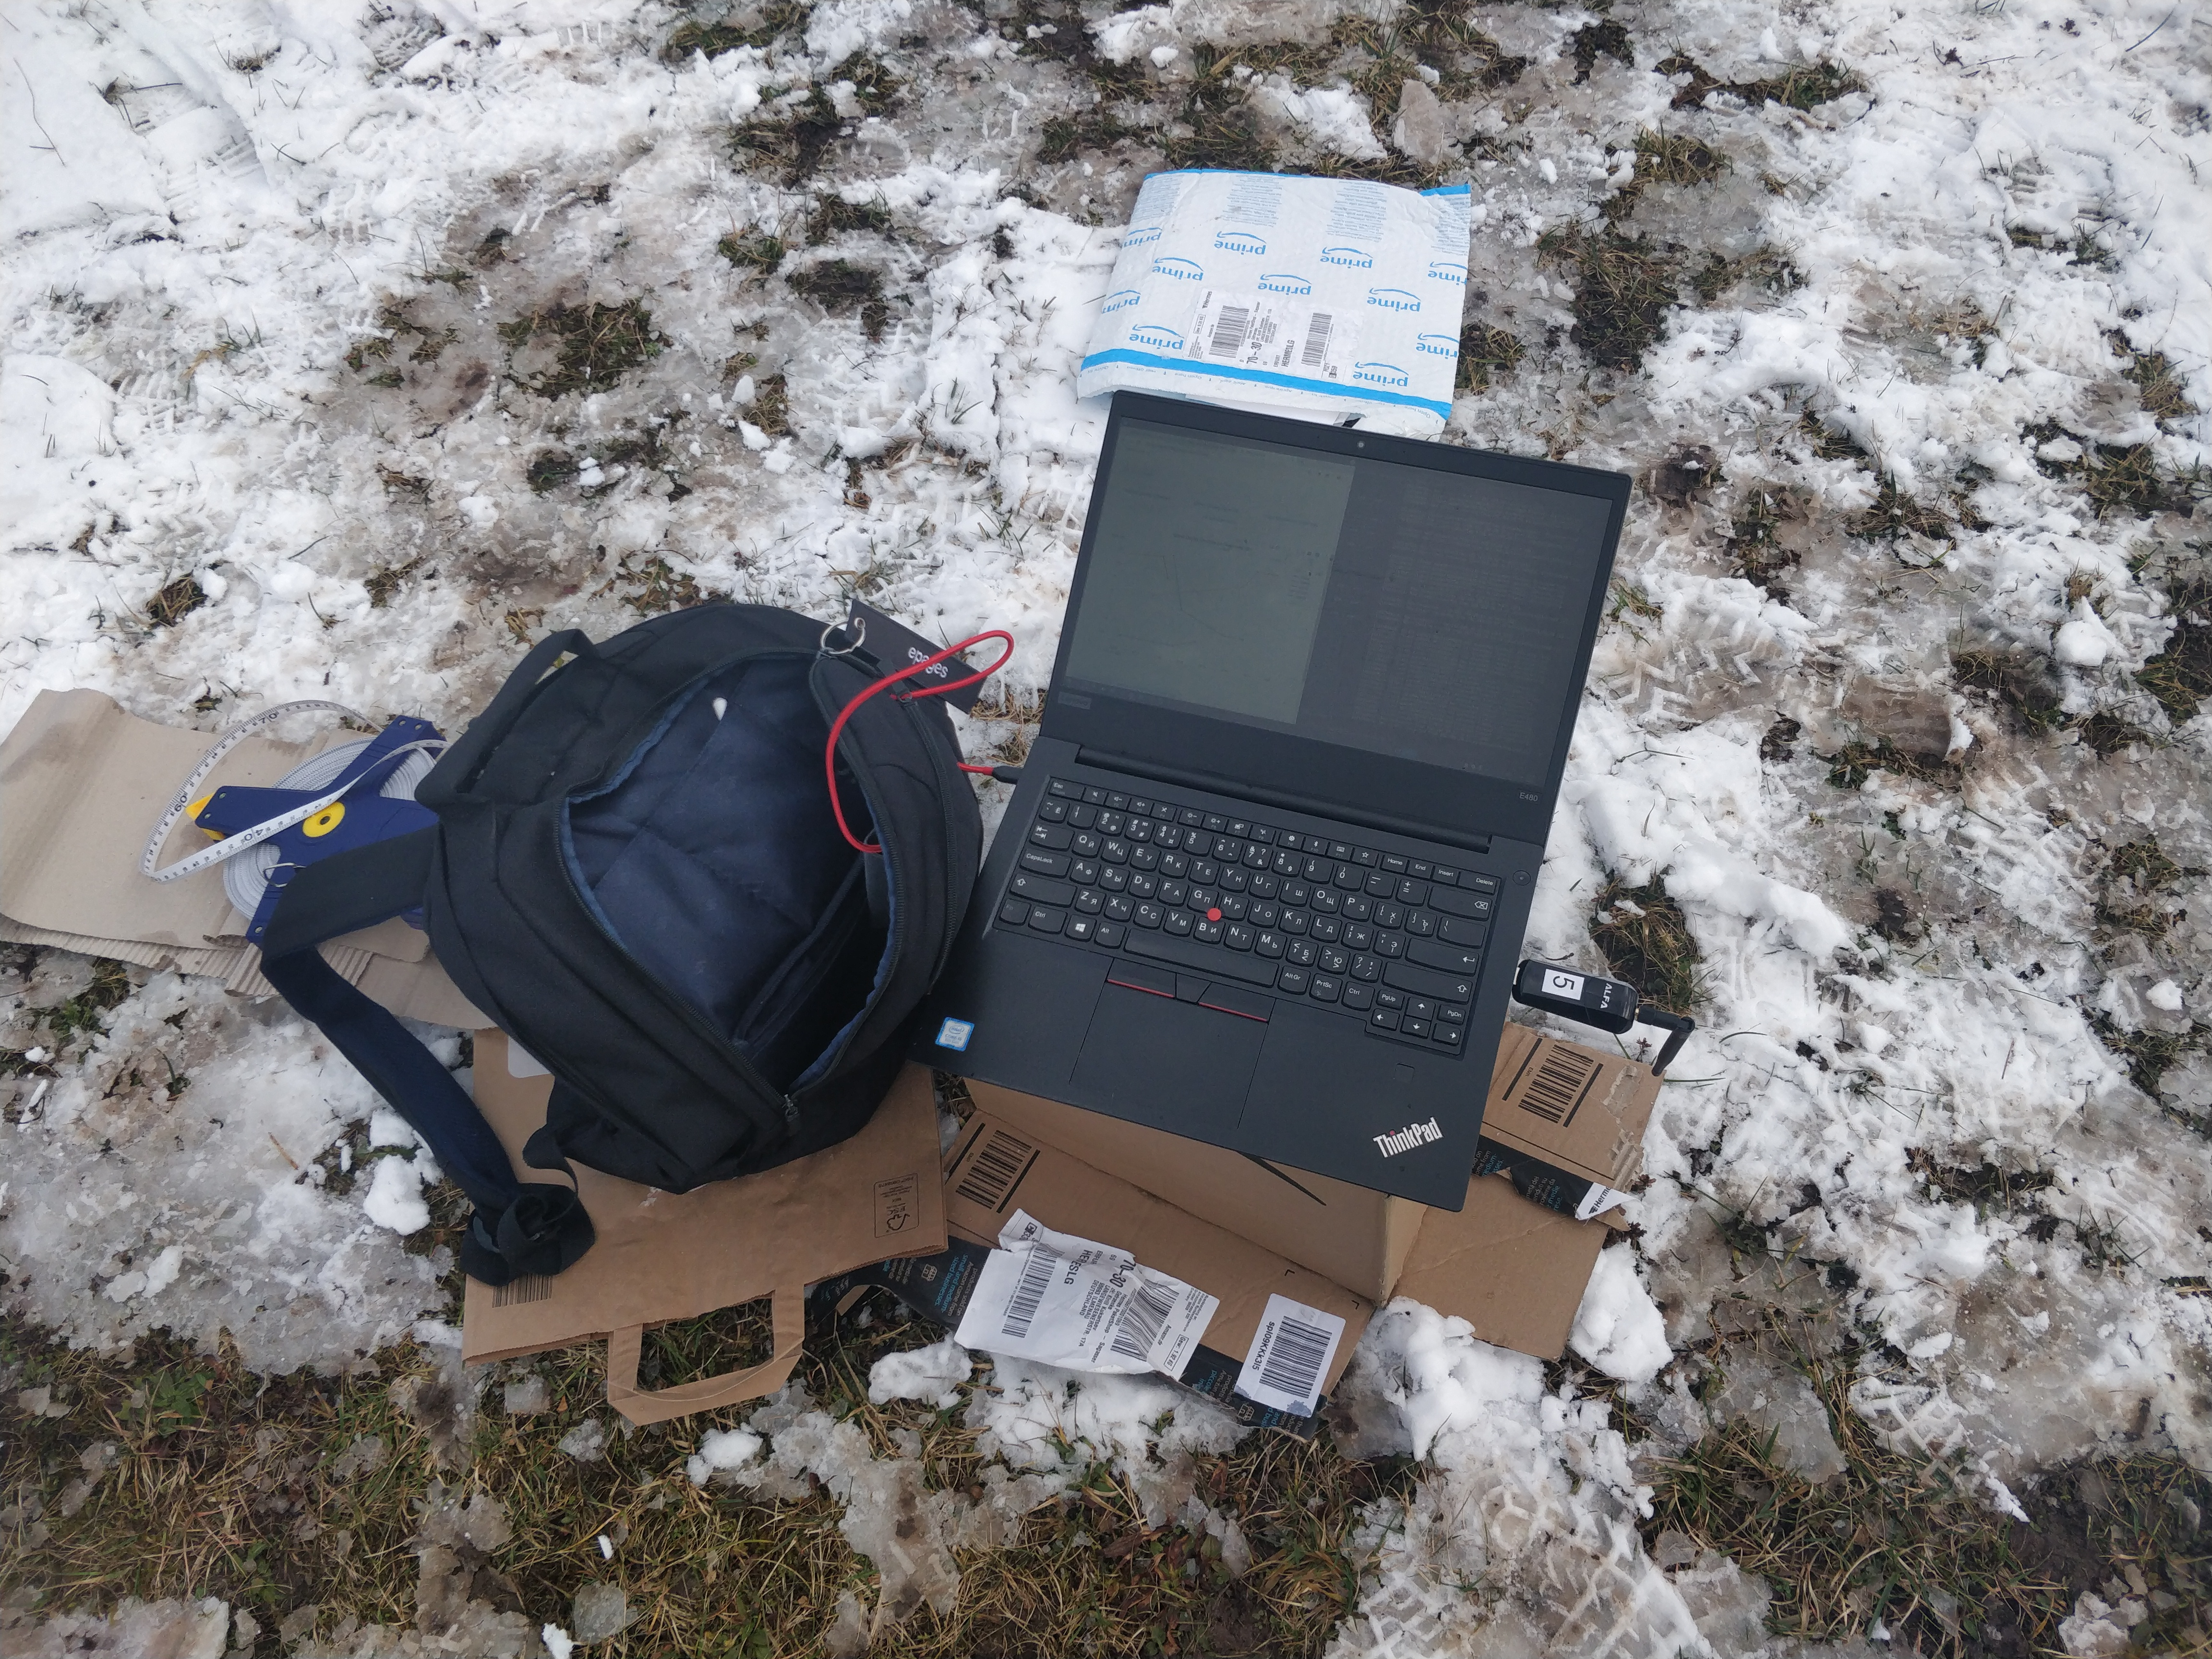
\includegraphics[width=\linewidth,keepaspectratio]{images/experiment_1_cnc.jpg}
\caption{Layout of CnC server}
\end{figure}

\subsubsection{Case 1}

\textbf{Suboptimal scheme} was chosen to begin with: UEs' connection to one AP was made successfully.

The second AP was connected to the other 3 UEs with more effort. The reason for it was in the Wi-Fi module issues of AP  (the laptop freeze).

After some time of data collection, it was clear the second AP was not sending data to CnC at all, so we decided to locate devices according to the near-optimal scheme.

\subsubsection{Case 2}

This helped to increase the RSS level a bit from -82 and -84 to -76 and
-80, data still was collected only from the first AP.

Besides, the graphical view in CnC showed 4 UEs close to each other (having approximately the same GPS coordinate), whereas the other 2 were detected much further.

Then we figured out that the second AP stopped working at some time. Restart and re-connection of UEs did not help to obtain data of that 3 UEs in CnC.

\subsubsection{Case 3}

It made no sense to try without data collection on CnC.

\subsection{Outcome}

The first attempt of the experiment showed:

\begin{itemize}
\tightlist
\item
  Further development of GPS\_Tracker and GPS\_Android to fix bugs required.
\item
  Tests of placement algorithms performing, but due to problem with message communication, we were unable to test if the optimized positions would lead to better signal conditions.
\end{itemize}

As a result, we decided to:

\begin{itemize}
\tightlist
\item
  fix the second AP failure reasons
\item
  figure out the source of 2 point-outliers in the plot
\end{itemize}
